\subsection{UC-5}

\begin{figure}[H]
    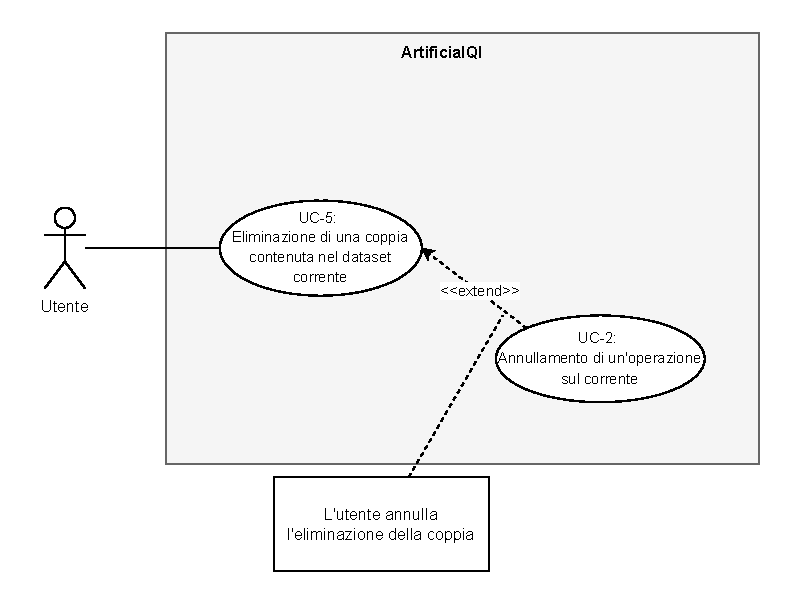
\includegraphics{Sezioni/UseCase/Immagini/UC-5.pdf}
    \caption{Diagramma UC-5.}
\end{figure}

\begin{usecase}{UC-5}{Eliminazione di una coppia contenuta nel dataset caricato}
    
    \req{\hyperref[item:RU-1]{RU-1}} 

    \pre{
        \item Il sistema è attivo e funzionante
        \item La coppia da eliminare è contenuta nel dataset caricato
    }

    \post{
        \item La coppia viene eliminata dal dataset caricato
    }
    
    \actor{Utente}

    \subactors{}

    \trigger{L'utente deve eliminare una coppia contenuta nel dataset caricato}
    
    \inc{}

    \base{}

    \scenario{
        \item L'utente richiede l'eliminazione di una coppia contenuta nel dataset caricato
        \item L'utente conferma l'eliminazione
        \item La coppia viene eliminata dal dataset caricato
    }

    \subscenario{
        \item[2.1] \textbf{L'utente annulla l'eliminazione della coppia:} 
        \begin{itemize}
            \item[a.] \hyperref[subsec:UC-2]{UC-2}
        \end{itemize}
    }
\end{usecase}
